Unser Prototyp setzt sich derzeit aus 3 Systemen zusammen: dem Arduino samt Shield für die Möglichkeit der Ortung und Simkartenslot, den Webserver zur Datenverteilung und -bereitstellung sowie eine App für die Smartphone Betriebssysteme Android und iOS.

\textbf{Bild (Raspi, Arduino, Smartphones mit geöffneter App)}

\section{zukünftiges Produktangebot}
Wir haben uns zwei Produktkategorien überlegt, mit denen wir Gewinn generieren können. Zum einen ist das ein monatliches Bezahlkonzept. Hierbei haben wir uns an dem Konzept einiger Mobilfunkanbieter orientiert. Die Überlegung ist, dass wir zwei hinzu buchbare Optionen anbieten und man nur das bezahlt, was wirklich gebraucht wird. Eine Optionen ist die Google Standort API für eine genauere und zuverlässigere Standorterkennung. Die andere Option ist das Bestellen einer Sim-Karte mit Mobilfunkvertrag. Die Idee ist hier, dass so gegen einen kleinen Aufpreis der Ease-of-Use unseres Produkts weiter gesteigert wird.

Für das Endgerät haben wir uns neben der aktuellen Basis Variante für eine Base+ und eine Pro Variante entschieden. Bei der Base+ Variante ergänzen wir die Basis Variante lediglich um eine Sirene und etwas mehr Akkuleistung. Für die Pro Variante erweitern wir das Basismodell um einen WLAN Empfänger. Des Weiteren überlegen wir unseren modularen Aufbau für eine weitere Umsatzsteigerung zu nutzen und Akkumodule zu verkaufen, mit denen die Akkulaufzeit unserer Produkte vom Nutzer beliebig verlängert werden kann. Ein weiterer Vorteil ist, dass so bei nachlassender Akkuleistung unser Produkt nicht entsorgt werden muss, sondern der Nutzer einfach mit offiziellen Produkten den Akku wechseln kann. Dies soll verhindern, dass der Kunde auf Drittanbieter zurückgreift.
Das Ziel ist, dass wir unsere Apps und den Webserver unabhängig von der Produktversion verwenden können.

\section{Vergleich} 
Eine kurze Suche im Internet nach ähnlich funktionierenden  Systemen lässt schnell die Frage aufkommen : 
Wo liegt bei uns der Unterschied?
Für die direkte Konkurrenzanalyse haben wir uns für den Platzhirsch Amazon entschieden, da es wahrscheinlich nirgendwo sonst so viele ähnliche Produkte aus den unterschiedlichsten Ländern mit diversen Qualitätsmerkmalen gibt. Wir haben dafür Produkte im niedrigeren  Preissegment für rund 30€, im mittleren für rund 60€ und im höherpreisigen für weit über 100€ mit unserem verglichen. 

\begin{figure} [H]
	\begin{center}
		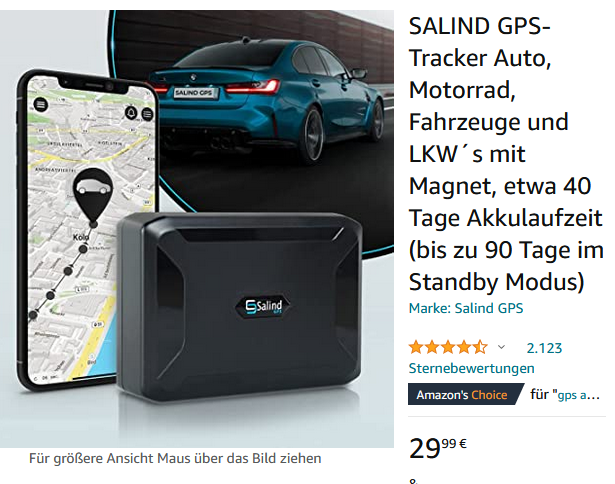
\includegraphics[width=0.75\textwidth]{Bilder/Produkt_Vergleich.png}
		\caption{Vergleichsprodukt im unteren Preissegment}
		\cite{Salind}
		\label{product_vgl}
	\end{center}
\end{figure}

Es lässt sich festhalten, dass alle Systeme die gleiche Grundfunktion besitzen: eine App, mit der das sich im Auto befindliche Gerät über einen Server Koordinaten-Daten abrufen und auswerten kann. Dennoch sind uns wesentliche Punkte aufgefallen, die sich abheben:

\begin{itemize}
	\item unser System ist nicht fest in sich verbaut, das bedeutet bei möglichen Defekten kann es leicht geöffnet werden und bei Bedarf einfach selbstständig repariert werden
	\item Die Akkus sind austauschbar und können mit einem handelsüblichen Ladegerät bequem daheim aufgeladen werden, so muss das Gesamtsystem nicht aus dem Auto entnommen werden. Anmerkung: alle Systeme, die wir uns angesehen haben, haben festverbaute Akku Systeme, die nur über Micro USB aufgeladen werden können
	\item Aus diesen Punkten ergibt sich auch direkt der nächste positive Effekt: da alle Bestandteile leicht zugänglich und austauschbar sind, ist unser Produkt sehr viel nachhaltiger - zudem haben wir auf unnötige Kunststoff Bestandteile verzichtet
	\item Des weiteren ist unser System durch sein offenherziges Design leicht erweiterbar und erinnert so unter anderem an die Uridee des \textit{Fairphone} mit seiner Komponenten Bauweise: man kauft nur, was man braucht, erhält aber garantiert ein funktionierendes Basissystem.
	\item Ebenfalls geht man bei unserem Produkt keine aufgezwungene Vertragspartner Bindung ein - der Internetanbieter kann sich der Kunde selbst aussuchen
\end{itemize}
Es lässt sich daher behaupten - Ja, Produkte wie dieses sind in der Basis nicht neu, dennoch haben wir uns Gedanken in ganz unterschiedliche Richtungen gemacht und unseren Ideenhorizont frei gehalten, so dass sich unser Produkt stetig mit und für den Kunden weiterentwickeln kann.
